\section{Aufbau}
Zum Sammeln von Daten von Twitter verwenden wir einen Crawler, welcher über die Twitter-API Daten sammelt. Dazu ist es nötig diese Daten zu empfangen, dann zu puffern und schlussendlich in die Datenbank zu Schreiben. Allerdings müssen die Daten noch gefiltert werden, da wir nur Daten von verifizierten Twitter-Accounts (und manuell hinzugefügten) speichern. Sind die Daten gefiltert, werden sie vom Crawler noch lokalisiert. Das heißt, dass jedem Account beziehungsweise jedem Retweet eine Geoposition/Land zugeordnet wird. Ist dies erfolgt so werden die Daten in die Datenbank geschrieben.
\\ In \cref{fig:uml_crawler} ist der Aufbau des Crawlers anhand eines UML-Klassendiagramms spezifiziert.

\begin{figure}[h!]
	\centering
	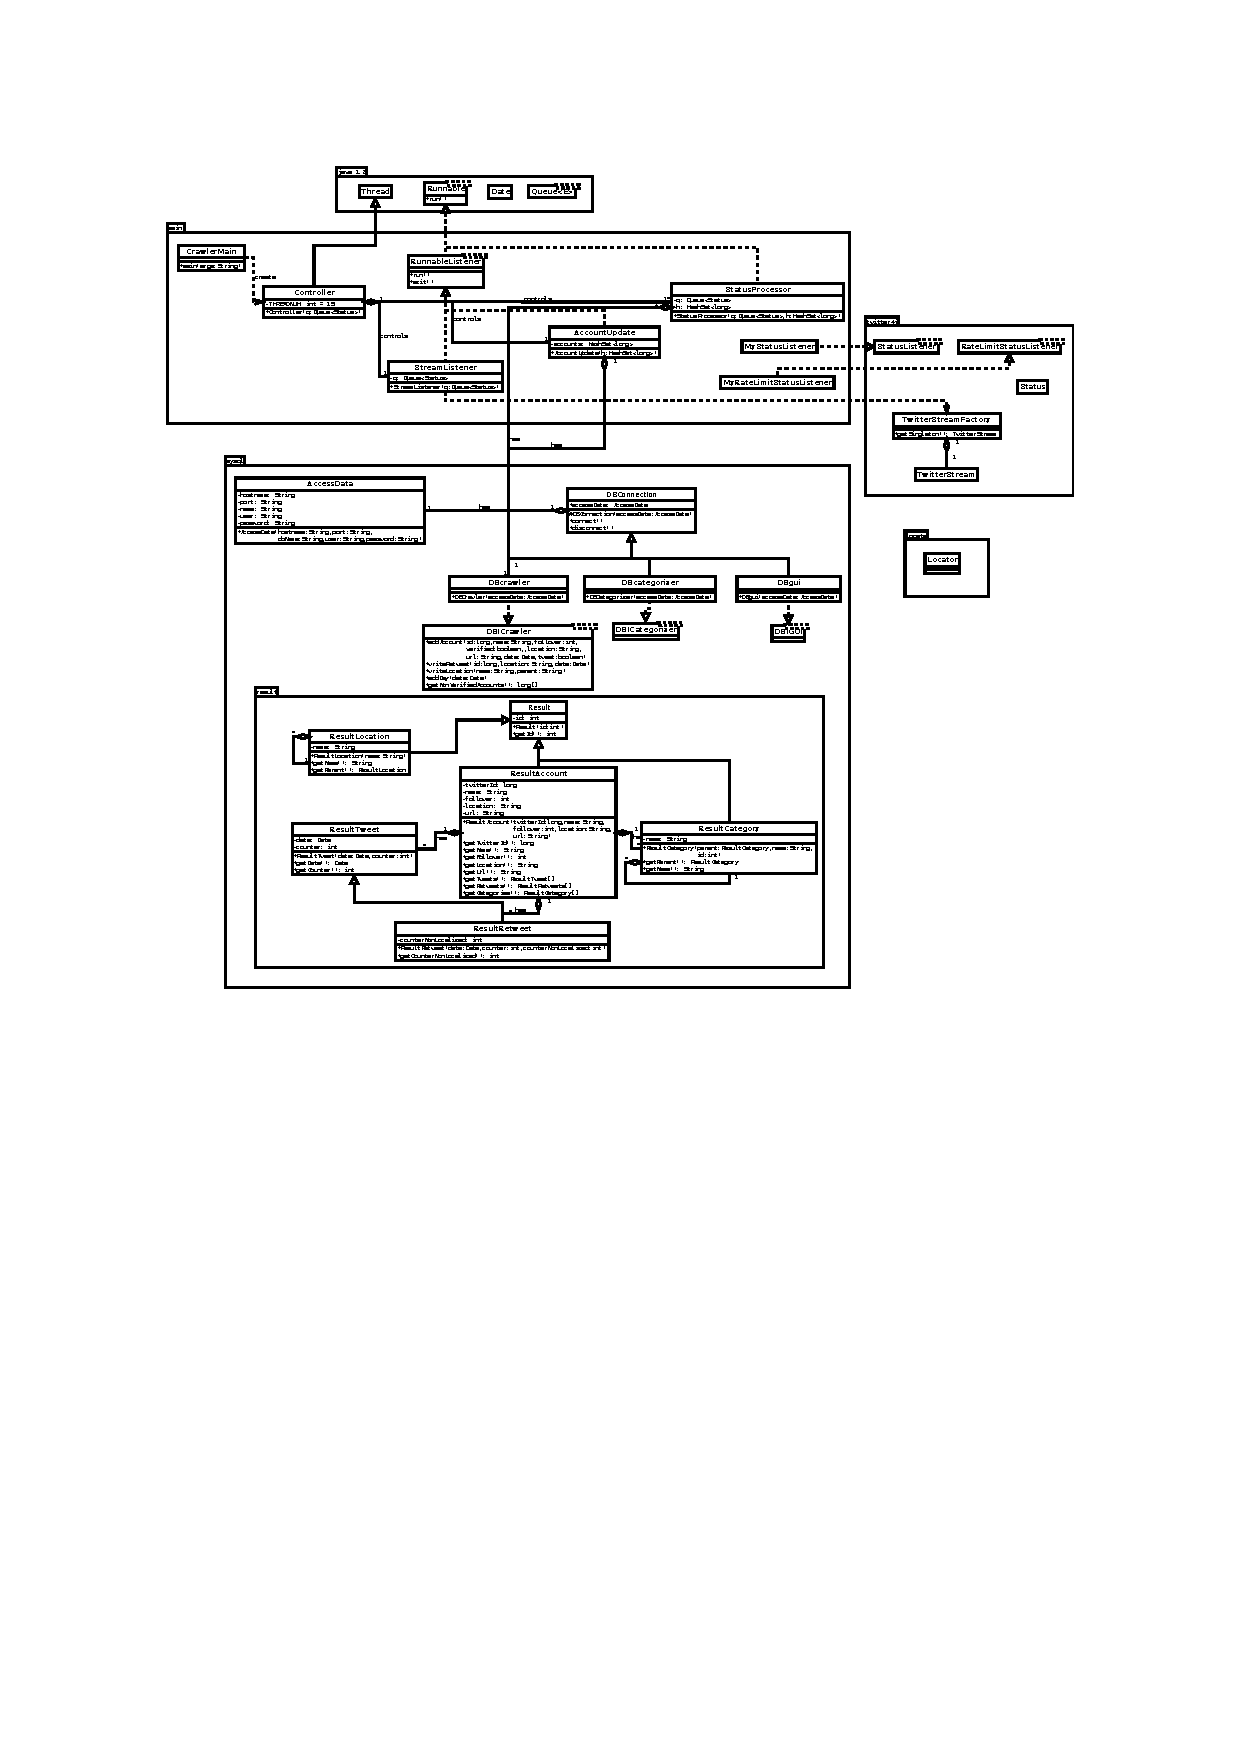
\includegraphics[width=\textheight,height=\textwidth,keepaspectratio=true,angle=-90]{dia/uml_crawler}
	\caption{UML-Klassendiagramm des Crawlers}
	\label{fig:uml_crawler}
\end{figure}

\begin{description}
\item[CrawlerMain] Klasse dient als Einstieg ins Programm. Sie überprüft die Eingabe für die Datenbankverbindung und startet einen Controller. Danach seht sie dem Benutzer über die Konsole zur Verfügung um das Programm zu überwachen.
\item[RunnableListener] Interface welches Runnable erweitert und zusätzlich noch eine exit-Methode fordert um Threads zu beenden.
\item[Controller] Diese Klasse koordiniert alle Aktionen die nötig sind um Daten bei Twitter abzuholen und in die Datenbank zu Schreiben. Dazu startet sie einen StreamListener, ein AccountUpdate und mehrere StatusProcessor's jeweils als Thread. Außerdem kontrolliert sie den Puffer und sorgt für ein sauberes Beenden des Programms indem alle Verbindungen ordnungsgemäß geschlossen und die Threads beendet werden.
\item[StreamListener] Stellt eine Verbindung zur Twitter-Streaming-API her und initialisiert einen MyStatusListener.
\item[AccountUpdate] Diese Klasse stellt eine Methode zur Verfügung um in der Datenbank periodisch nach Accounts zu suchen, welche manuell hinzugefügt wurden, aber auch wie Verifizierte behandelt werden sollen.
\item[StatusProcessor] Diese Klasse stellt die Funktionalität zur Filterung der Daten von Twitter zur Verfügung, welche sie aus dem Puffer nimmt. Außerdem bietet sie die Möglichkeit diese Daten in die Datenbank zu schreiben.
\item[MyStatusListener] Diese Klasse nimmt die Daten von Twitter entgegen und schreibt diese in einen Puffer.
\item[MyRateLimitStatusListener] Diese Klasse nimmt Meldungen von Twitter bezüglich RateLimits entgegen.
\item[Locator] Der Locator lokalisiert Accounts und Retweets mithilfe eines Webdienstes.
\end{description}

\section{Start des Crawlers}
Beim Starten des Crawlers werden sämtliche notwendigen Komponenten der Reihe nach gestartet. Dadurch wird garantiert, dass jede Komponente eine Umgebung vorfindet in der sie laufen kann und alle Ressourcen bereits zur Verfügung stehen. In \cref{fig:crawler_start} ist der Start des Crawlers beispielhaft mit 2 StatusProcessor's dargestellt.

\begin{figure}[h!]
	\centering
	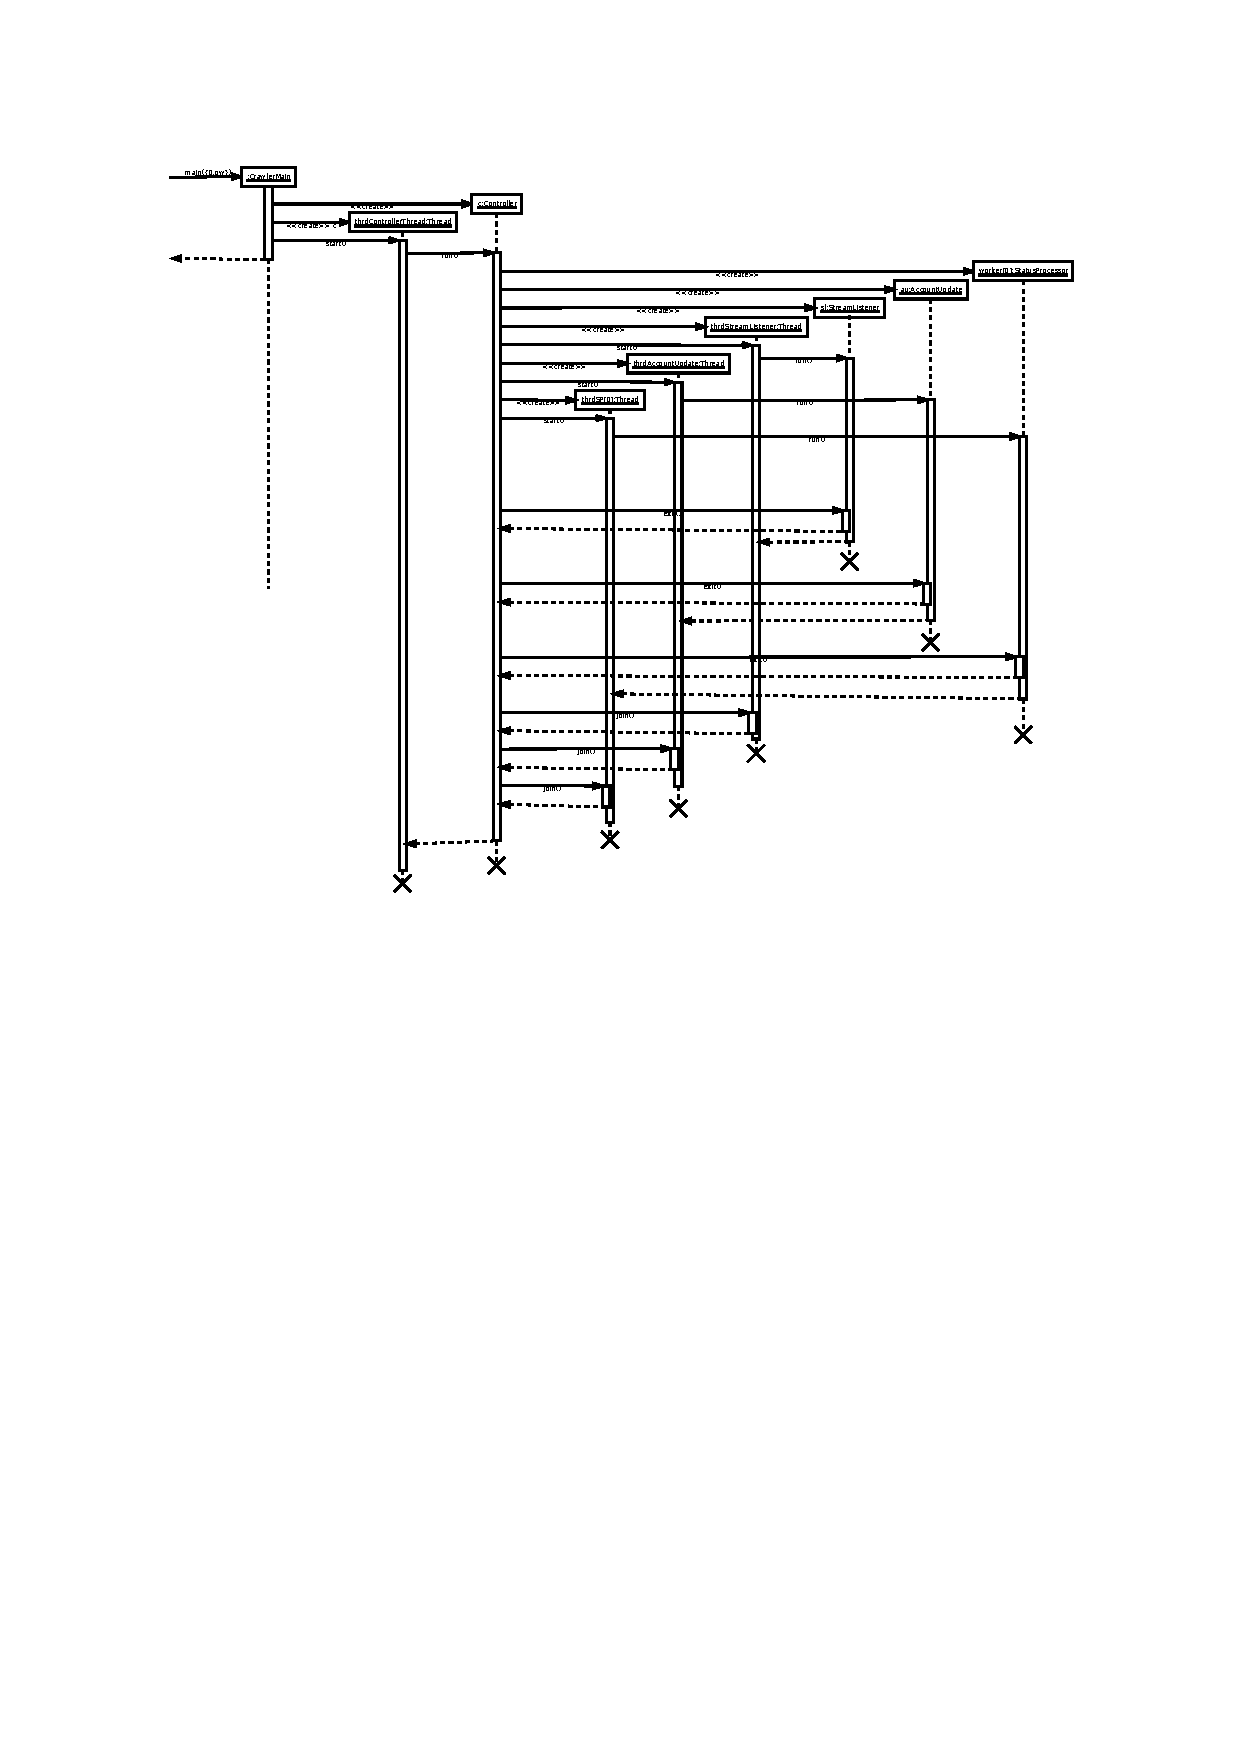
\includegraphics[width=\textheight,height=\textwidth,keepaspectratio=true,angle=-90]{dia/crawler_start_sequence}
	\caption{Sequenzdiagramm zum Start des Crawlers}
	\label{fig:crawler_start}
\end{figure}

Um den Crawler zu starten, werden ihm die Zugriffsdaten auf die Datenbank übergeben und die Anzahl der Threads die später Daten verarbeiten (Hardware abhängig).
Die main-Methode der Main-Klasse instantiiert daraufhin ein Controller Objekt, welches ab dann sämtliche Steuerung übernimmt. Diese Controller Objekt wird dann in einem Thread ausgeführt. Die Main-Klasse ist nun nur noch dafür zuständig Benutzereingaben entgegenzunehmen und weiter zu delegieren.
Sobald der Controller gestartet wurde instantiiert er die StatusProcessor Objekte, welche später sämtliche Daten verarbeiten müssen (deren Anzahl vom Benutzer festgelegt wird). Außerdem werden noch ein AccountUpdate- und ein StreamListener-Objekt instantiiert. Ersteres dient dazu eine Liste nicht verifizierter Accounts, die dennoch getracked werden sollen, aus der Datenbank aktuell zu halten. Zweiteres ist dafür zuständig eine Verbindung zur TwitterStream-API einzurichten. Alle diese Objekte werden dann vom Controller als eigenständige Threads ausgeführt.
Daraufhin beginnt der StreamListener eine Verbindung zur TwitterStreaming-API herzustellen (siehe \cref{fig:initialize_stream}).\\
Nun ist der Crawler im aktiven Zustand und empfängt Daten von Twitter, welche dann gefiltert, vervollständigt und in der Datenbank abgelegt werden.\\
Wird der Crawler vom Benutzer beendet, so sendet der Controller jedem Objekt, welches in einem Thread läuftein exit-Signal. Daraufhin beenden die Objekte ihre Tätigkeit und der jeweilige Thread kehrt zum Controller zurück, sodass dieser dann das gesamte Programm beenden kann.
\\

\begin{figure}[h!]
	\centering
	\includegraphics[width=\textheight,height=\textwidth,keepaspectratio=true,angle=-90]{dia/crawler_initialize_stream}
	\caption{Sequenzdiagramm zur Initialisierung des TwitterStreams}
	\label{fig:initialize_stream}
\end{figure}

Um eine Verbindung zur Twitter-Streaming-API herzustellen, wird zuerst ein RateLimitStatusListener erstellt um auf Rate-Limits von Twitter zu reagieren. Danach wird noch ein Filter erstellt mit dem der Twitterstream durchsucht wird und ein MyStatusListener um über eingehende Daten benachrichtigt zu werden.
Anschließend wird ein TwitterStream-Objekt aus der twitter4j-Bibliothek geholt(ist Singleton). Auf diesem werden dann die Methoden zur Initialisierung aufgerufen und somit die Listener und der Filter gesetzt.\\
Zum Schließen des Streams wird auf dem TwitterStrem-Objekt die shutdown-Methode aufgerufen.

\section{Verarbeitung der Daten von Twitter}
Um zu verdeutlichen wie die Daten von Twitter innerhalb des Crawlers verarbeitet werden, ist in \cref{fig:crawler_process} der Datenfluss durch den Crawler exemplarisch dargestellt. Dabei werden die Daten von Twitter abgeholt, gepuffert, dann gefiltert und schlussendlich in die Datenbank geschrieben.

\begin{figure}[h!]
	\centering
	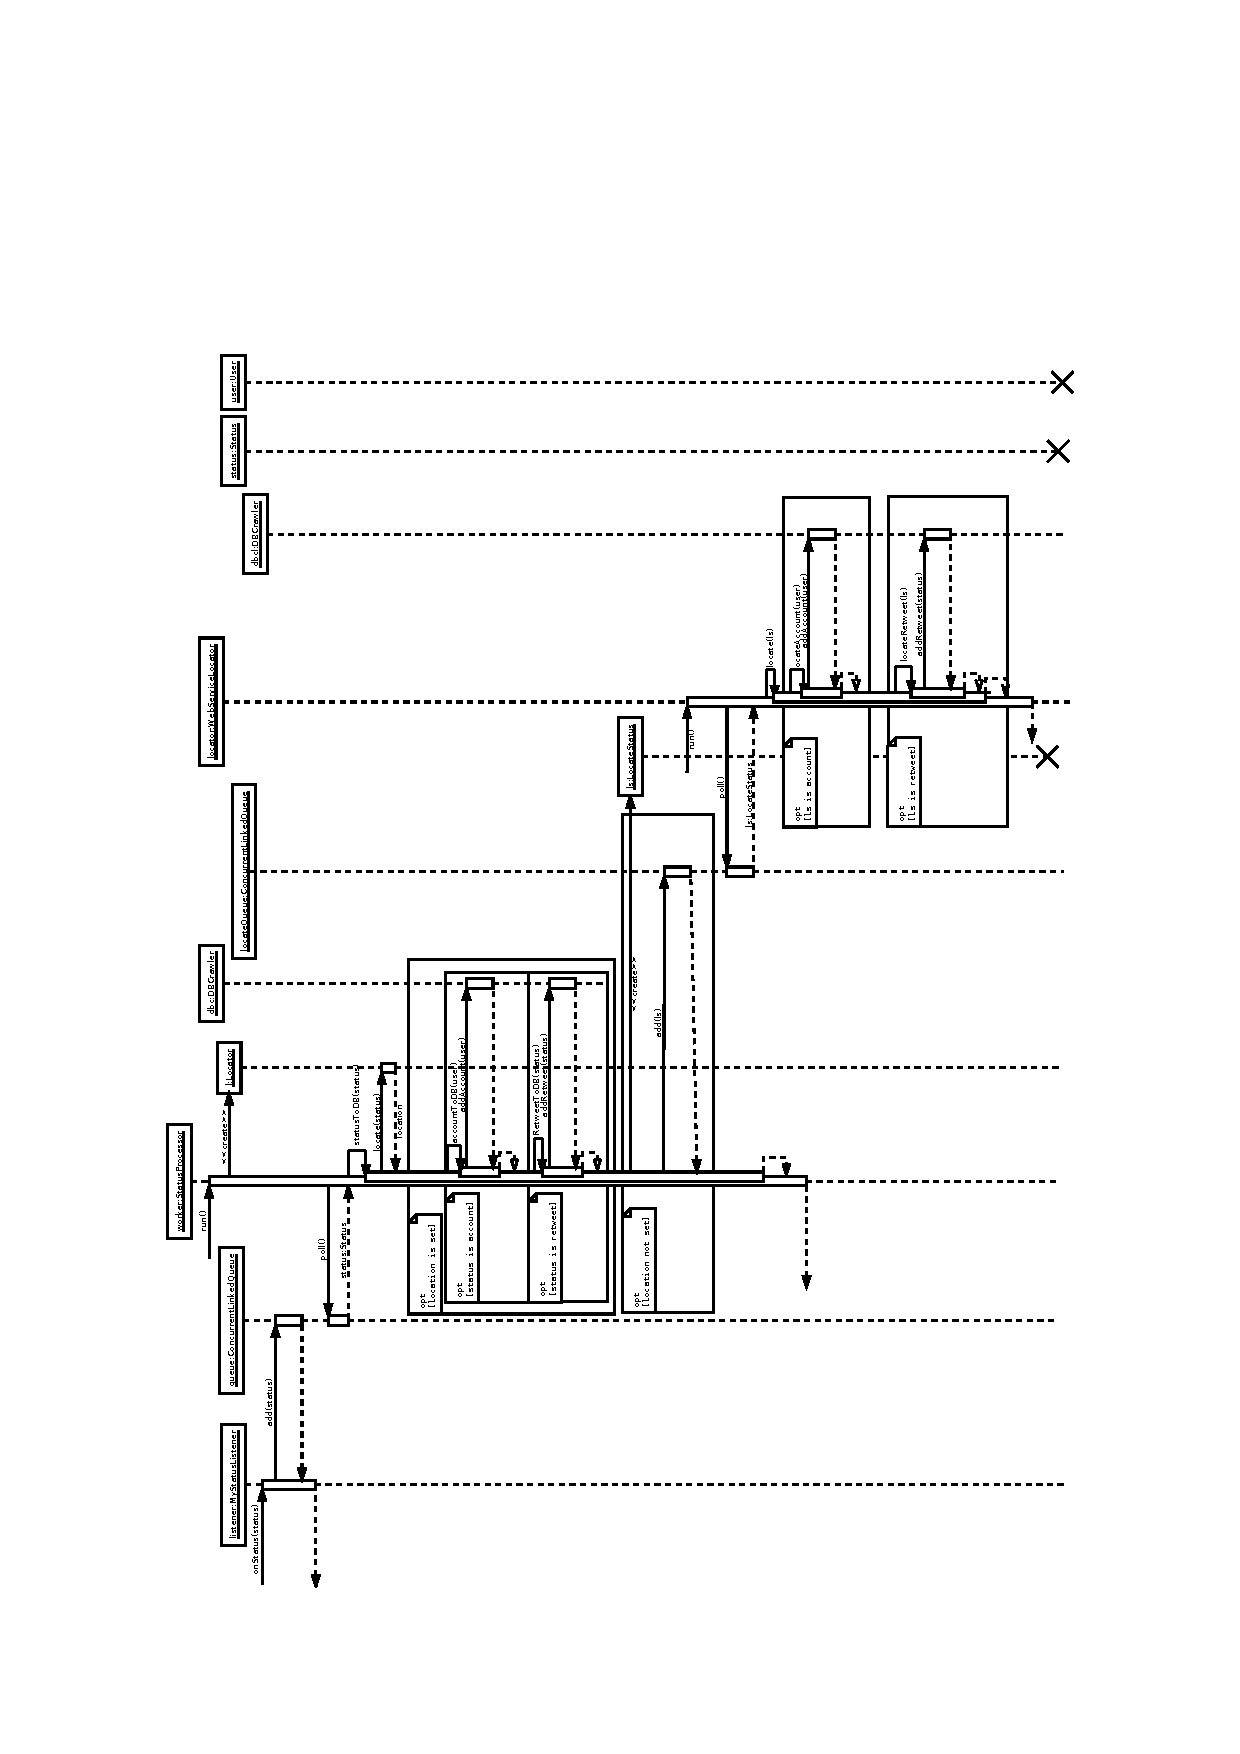
\includegraphics[width=\textheight,height=\textwidth,keepaspectratio=true,angle=-90]{dia/crawler_process_sequence}
	\caption{Sequenzdiagramm der Verarbeitung der Daten von Twitter}
	\label{fig:crawler_process}
\end{figure}

Im Folgenden soll der Weg der Daten von Twitter in unsere Datenbank mit \cref{fig:crawler_process} beschrieben werden.
Zuerst werden die Daten, welche im MyStatusListener auflaufen in eine (threadsichere) Warteschlange geschoben.
Hat dann ein StatusProcessor freie Kapazitäten so entnimmt er das erste Element der Warteschlange. Dieses Status-Objekt enthält alle relevanten Informationen um zu entscheiden ob das Objekt interessant ist oder nicht.
Interessante Status-Objekte enthalten verifizierte Twitter-Accounts oder Retweets auf Tweets von verifizierten Accounts. Ist ein verifizierter Account in einem Status-Objekt gefunden worden, so wird der Account (hier: user) dem Locator zur Lokalisierung übergeben. Dieser versucht dann anhand eines Orts-Strings den Account einem Land zuzuordnen. Ist dies geschehen so wird der Account in die Datenbank geschrieben. Genauso wird auch mit den Status-Objekten verfahren die einen Retweet enthalten.
Ist ein solches Status-Objekt verarbeitet, so beginnt der ganze Verarbeitungsprozess wieder von vorne.